\chapter{Rapidly-Exploring Random Tree}\label{chap:RRT}

\section{General}

The goal of this thesis is not only to generate a numerically stable, snap optimized polynomial trajectory but also to explore a densely packed (indoor) environment and plan an aggressive trajectory in between the obstacles. Hence, the Rapidly-Exploring Random Tree (RRT) algorithm is used to find a collision-free straight line solution through densely packed environments. The sampling points of the RRT (or RRT*) algorithm are then used as the vertices in the polynomial optimization.

\section{RRT Algorithm}\label{sec:RRT}

RRT is a computational efficient algorithm to find a path in a high dimensional space by randomly building a space-filling tree. The sampling points are drawn randomly from the sample space and the tree grows incrementally. 
For each new sample the algorithm attempts to build a collision-free connection to the nearest state in the tree. If a collision-free connection is possible, the sample and the connection are added to the tree. \newline

An iteration of the RRT algorithm can be depicted schematically:

\begin{enumerate}
  \item Generate a random sample
  \item Find nearest state in tree
  \item Try to build a collision-free connection to the nearest state
  \item If feasible, add the sampled state and the connection to the tree
\end{enumerate}

\subsection{Goal State}

As mentioned above, the RRT algorithm is based on random samples. Therefore it is very unlikely that a sampled state perfectly matches the desired goal state. \newline
There are two different strategies to enable the RRT algorithm to get to the goal. One strategy is to define not only a goal state but a goal region. Every random sample which is located within the goal region is considered a goal state. As soon as a collision-free connection to a sample in the goal region is established, this trajectory is stored as the best trajectory. At this point the algorithm can be stopped or further iteration can be performed to find a better trajectory to the goal region. Once an other state from the goal region is sampled and the cost of the path to the new state is lower then the cost of the best trajectory, the best trajectory is replaced by the new path. \newline
Another strategy is to steer the RRT algorithm directly to the goal state. In addition to the randomly sampled states the exact goal state is added to the algorithm. The schematic description of an iteration of the RRT algorithm listed in section \ref{sec:RRT} can be modified to represent an iteration with the goal state:

\begin{enumerate}
  \item Insert goal state
  \item Find nearest state in tree
  \item Try to build a collision-free connection to the nearest state
  \item If feasible, add the sampled state and the connection to the tree
\end{enumerate}

In all the cases where a direct collision-free connection between start and goal state is not possible the iteration with the goal state will not succeed in a first attempt. Hence the iterations with the randomly sampled states described in section \ref{sec:RRT} are needed to build the space filling tree.\newline

Figure \ref{pic:smallGamma} depicts the straight line solution of the RRT algorithm with a fixed goal state. The figure is in bird's eye perspective and shows a crossing of different hallways. The blue cells represent the floor and the green cells represent the walls. The map was generated with a stereo camera and was not reworked. Therefore, some of the cells of the floor which should be occupied/blue are left free. 

\begin{figure}[H]
   \centering
   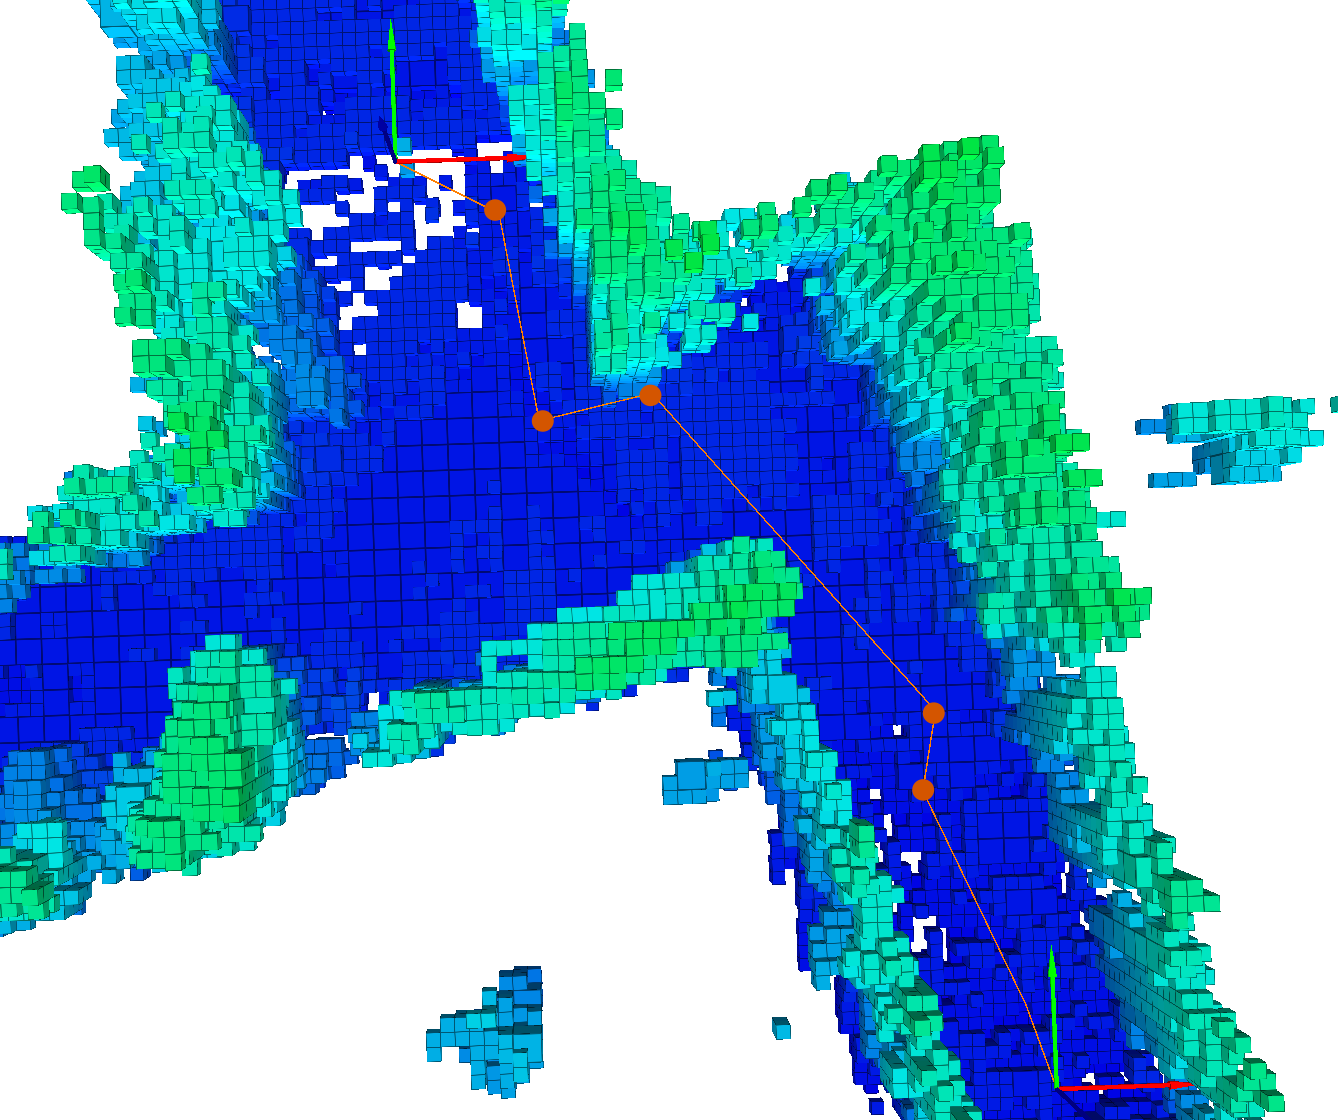
\includegraphics[trim = 50mm 0mm 30mm 0mm,clip,width=0.8\textwidth]{pics/smallGammaP.png}
   \caption{Straight line solution of the RRT algorithm with a fixed goal state. The start state (upper left corner) and the goal state are each represented by a $x$ and  $y$-vector. The random sampled states are depicted as orange dots.}
   \label{pic:smallGamma}
\end{figure}



\section{RRT* Algorithm}\label{sec:RRTstar}

In contrast to the RRT algorithm, the RRT* (or RRT Star) algorithm not only tries to connect to the nearest state in the tree but to several states near the sampled state. A user specified threshold defines which states of the tree belong to the "near states". If there is no state within the user specified range the algorithm attempts to build a collision-free connection to the nearest state in the tree just as the RRT algorithm would do.  \newline

The threshold, in our case the radius of a sphere, depends on an user-specified parameter $\gamma$. I.e. all the near states are located within this sphere. The radius $r$ can be calculated according to


\begin{equation}
r = \gamma * \left(\frac{ln(n+1)}{n+1}\right)^{1/d}
\label{equ:ballradius}
\end{equation}

where $n$ is the number of states which are already in the tree. The dimension of the state space $d$ is a fixed parameter and $ln$ represents the natural logarithm.\newline


As a first step, the sampled state is connected to the best state among the near states whereas "best" means minimum distance. Once the sampled state is added to the tree, all the other states among the set of near states are connected to the sampled state. If the connection is collision-free and the cost of the total path is smaller than the cost of the existing path, the old path is replaced. \newline

An iteration of the RRT* algorithm can be depicted schematically:


\begin{enumerate}
  \item Generate a random sample
  \item Define a threshold for a set of near states
  \item Try to build a collision-free connection to best state among the near states
  \item Add the sampled state and the connection to the tree 
  \item Try to connect all the other states from the set with the sampled state 
  \item Replace the old path if the new one has a smaller cost
  \item If there is no near state within the threshold, apply the RRT algorithm
\end{enumerate}


Because the RRT* algorithm tries to connect to several states each iteration, the procedure to find a path takes longer and is computationally more expensive. However, solutions with lower cost can be found by usning RRT* which is more important for most real life applications.

\subsection{Rewiring}\label{sec:Rewiring}


The sequence of step 5 and step 6 of the RRT* algorithm is called "rewiring".  As mentioned in section \ref{sec:RRTstar}, the RRT* algorithm is computationally more expensive but delivers trajectories with lower cost. Both aspects are caused by the rewiring and are therefore strongly influenced by the parameter $\gamma$ (equation \ref{equ:ballradius}). A large $\gamma$ defines a large sphere, hence it is likely to have more states (which are already in the tree) to be located within the sphere. The rewiring of the near states tends to result in shorter trajectories with fewer segments.\newline

Figure \ref{pic:smallBBX} depicts the straight line solution of the RRT* algorithm with a fixed goal state. Compared to figure \ref{pic:smallGamma}, a superior trajectory is found due to rewiring of the states in the tree.

\begin{figure}[H]
   \centering
   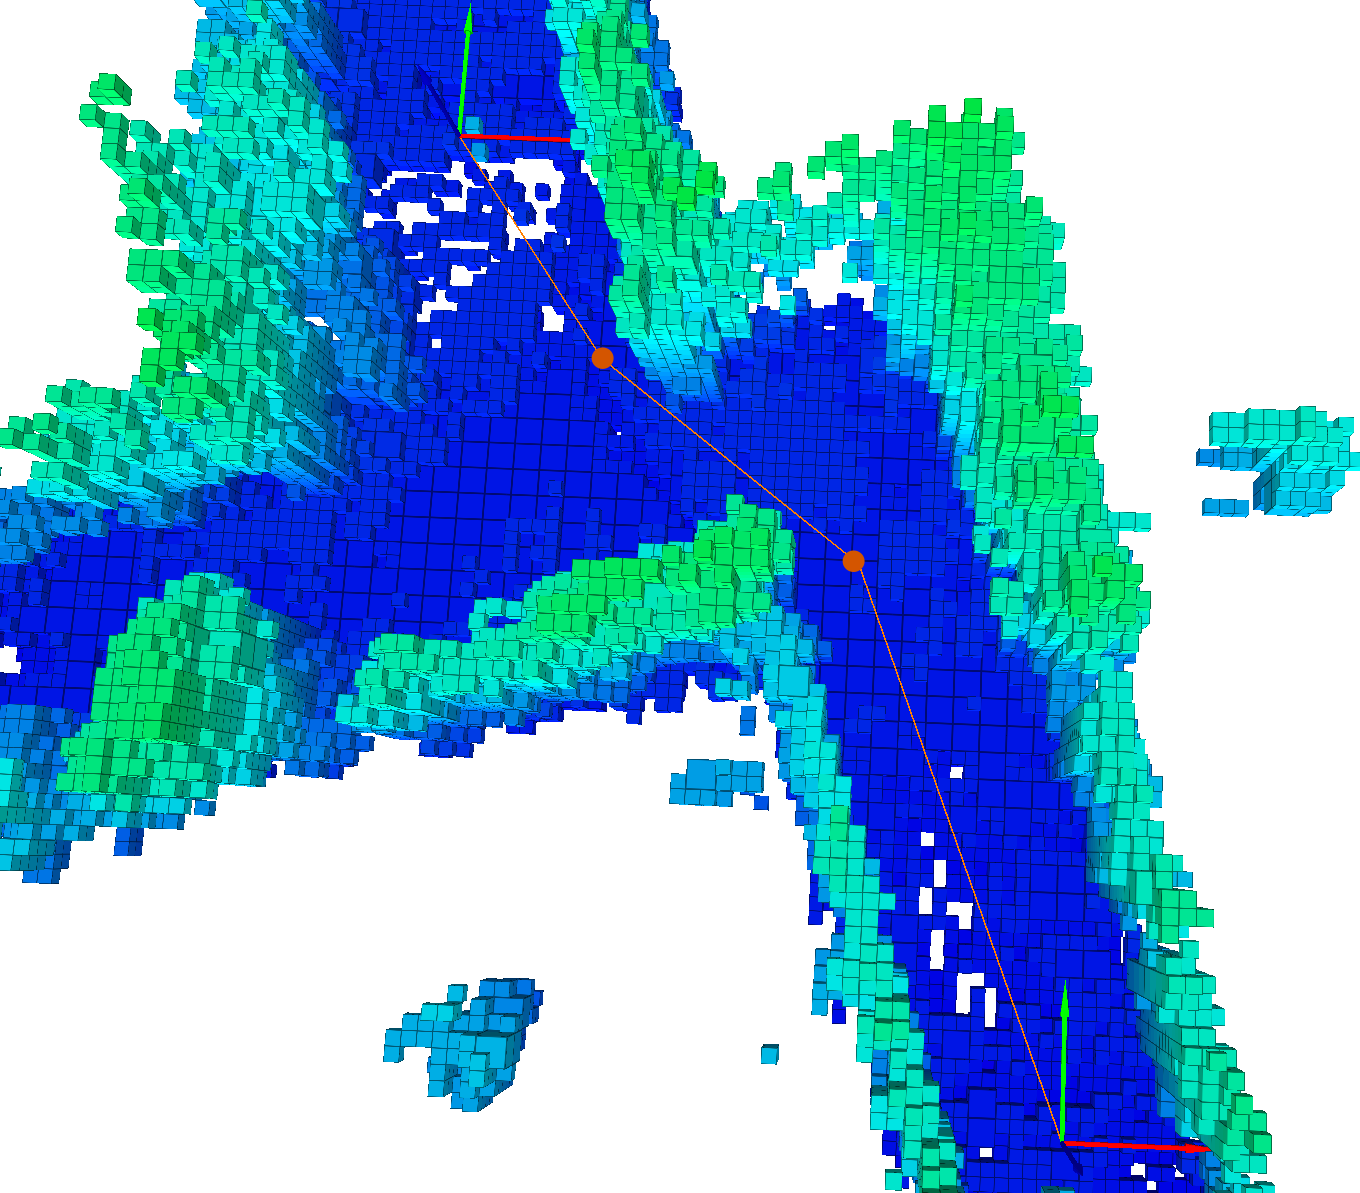
\includegraphics[trim = 50mm 0mm 30mm 0mm,clip,width=0.8\textwidth]{pics/smallBBXP.png}
   \caption{Straight line solution of the RRT* algorithm with a fixed goal state. The start state and the goal state are each represented by a $x$ and  $y$-vector. The random sampled states are depicted as orange dots. The $\gamma$ parameter in this example was set to $\gamma = 1.5$.}
   \label{pic:smallBBX}
\end{figure}


\subsection{Bounding Box}\label{sec:bbx}

The straight line solution in figure \ref{pic:smallBBX} is collision-free but very close to the walls. In real life application not only a point mass but a object (in this master thesis a UAV) should follow the trajectory. Therefore a bounding box needs to be installed around the trajectory. \newline
The bounding box is implemented as a cuboid. The 3 dimensions of the cuboid can be defined individually. The trajectory is then divided into a discrete trajectory and the bounding box is installed around the discrete points. If there is a obstacle in one of the bounding boxes the hole straight line is considered "in collision". \newline

Figure \ref{pic:bbx} depicts the straight line solution of the RRT* algorithm with a bounding box. In contrast to figure \ref{pic:smallBBX}, the trajectory is now located more central in the hallway because the bounding box makes it impossible to pass very close to the wall. Because the trajectory proceeds less direct from the start state to the goal state, the total distance of the trajectory increases. 

\begin{figure}[H]
   \centering
   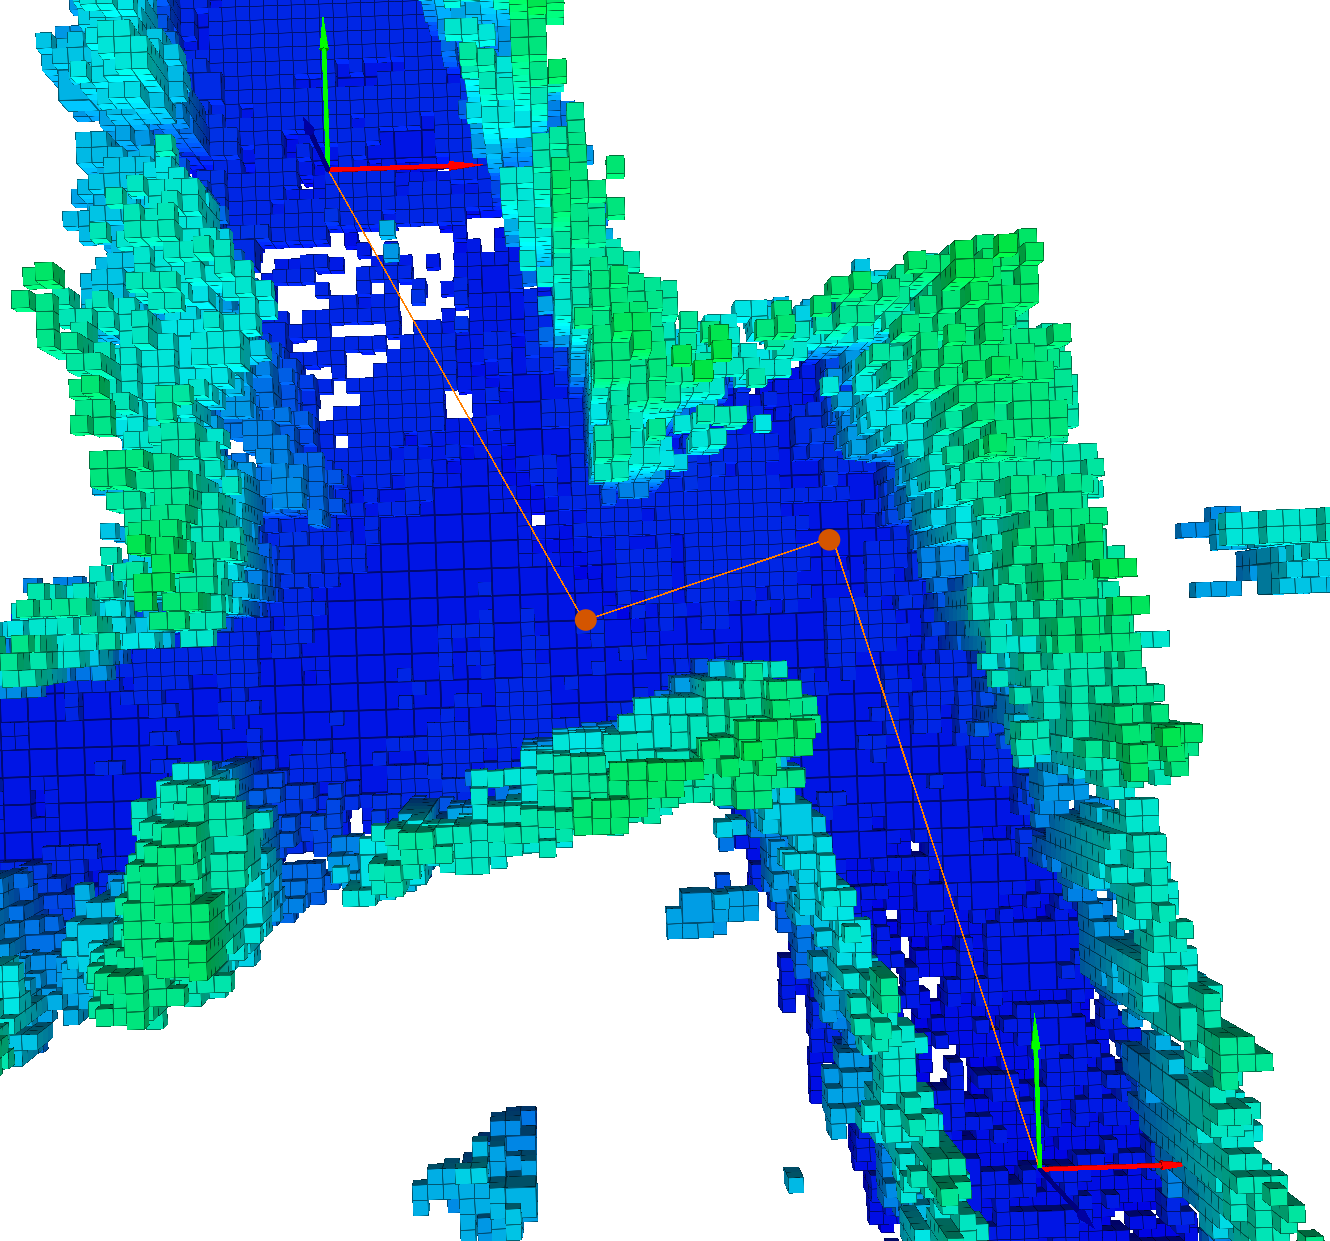
\includegraphics[trim = 50mm 0mm 30mm 0mm,clip,width=0.8\textwidth]{pics/largeBBXP.png}
   \caption{Straight line solution of the RRT* algorithm with bounding box. Due to the bounding box the trajectory is located more central in the hallway. The $\gamma$ parameter in this example was set to $\gamma = 1.5$.}
   \label{pic:bbx}
\end{figure}

\subsection{Ray Check}\label{sec:RayCheck}

Another approach to avoid collisions is the Ray Check method which is related to the concept of the "OctoMap" \cite{OctoMap}. In an OctoMap, the obstacles are stored as cells as can be seen in the figures above. Every cell has its individually key, which defines the location in the map. This keys are stored in a tree, named octree.\newline

As discussed in section \ref{sec:bbx}, a bounding box is used to check the trajectory for collisions. To do so, the trajectory is discretized and the bounding box is installed around every discrete trajectory-point. The bounding box is implemented as a cuboid with its edges aligned to the coordinate system of the map. Since the straight line connections can be situated arbitrary in space, a certain amount of overlap of the bounding boxes is required to guarantee that all the space around the trajectory is collision-free. As a downside of this overlap, several cells of the OctoMap are checked twice.\newline

To avoid the unnecessary double-check of the cells, a new approach called "Ray Check" is implemented. The idea is to generate a ray from one point in the OctoMap to another. Then, all the keys of the cells through which the trajectory passes are stored. Subsequently, the keys are checked if one of them represents an occupied cell. \newpage

Since a single ray does not represent any volume, multiple rays have to be tested. This corridor of rays is implemented as a tube in this master thesis.\newline

Figure \ref{pic:RayCheck} depicts the start of a straight line connection (red) which is situated arbitrary in space. Around the start point, a set of points is arranged on a circle. The same set of points have to be installed around the end point of the straight line connection (which is not depicted in figure \ref{pic:RayCheck}). If all the points around the start point are connected via a ray to the corresponding point around the end point, a tube develops.




\begin{figure}[h]
   \centering
   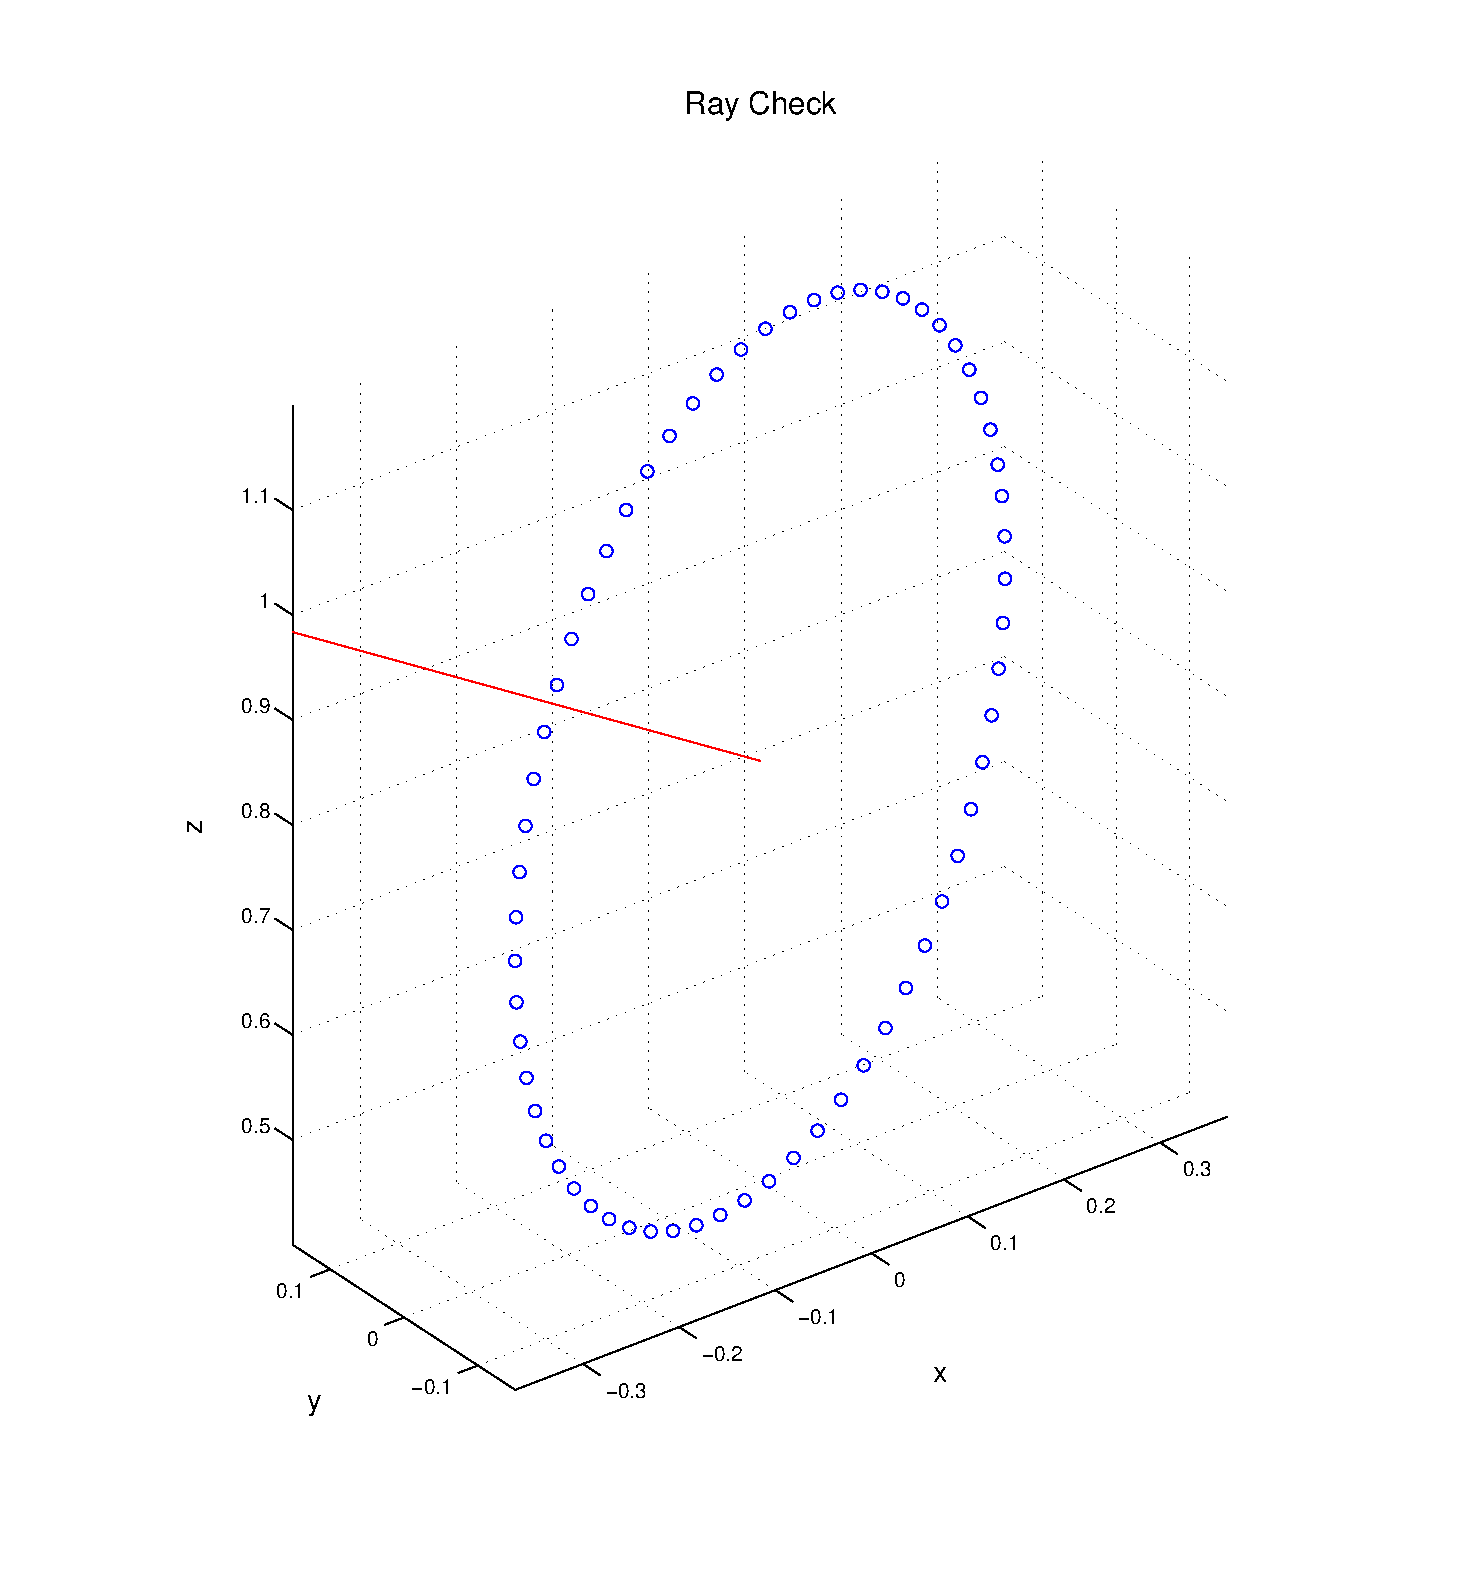
\includegraphics[trim = 25mm 10mm 30mm 10mm,clip,width=0.8\textwidth]{pics/RayCheck.eps}
   \caption{Points are arranged on a circle around the start point of a straight line connection. The points have to be connected to the corresponding point from the end point.}
   \label{pic:RayCheck}
\end{figure}

A problem with the Ray Check approach are floating objects. An object which is floating, i.e. has no connection to any wall, could be located inside the corridor without being touched by a ray. A lamp which hangs on a thin cable could lead to a floating object in the OctoMap if the cable is not detected.\newline

To resolve the problem, the OctoMap has either to be reworked or more points on different circles, each with a different radius, have to be added. Both possibilities would need additional computational time. \newline

First, the simple approach depicted in figure \ref{pic:RayCheck} is compared to the Bounding Box approach to decide if a further development of the Ray Check approach makes sense.
The two approaches have been tested for the start and goal point depicted in figure \ref{pic:differentGoalRRT}. The RRT* algorithm has been stopped as soon as a collision-free straight line solution was found. 

\begin{figure}[H]
   \centering
   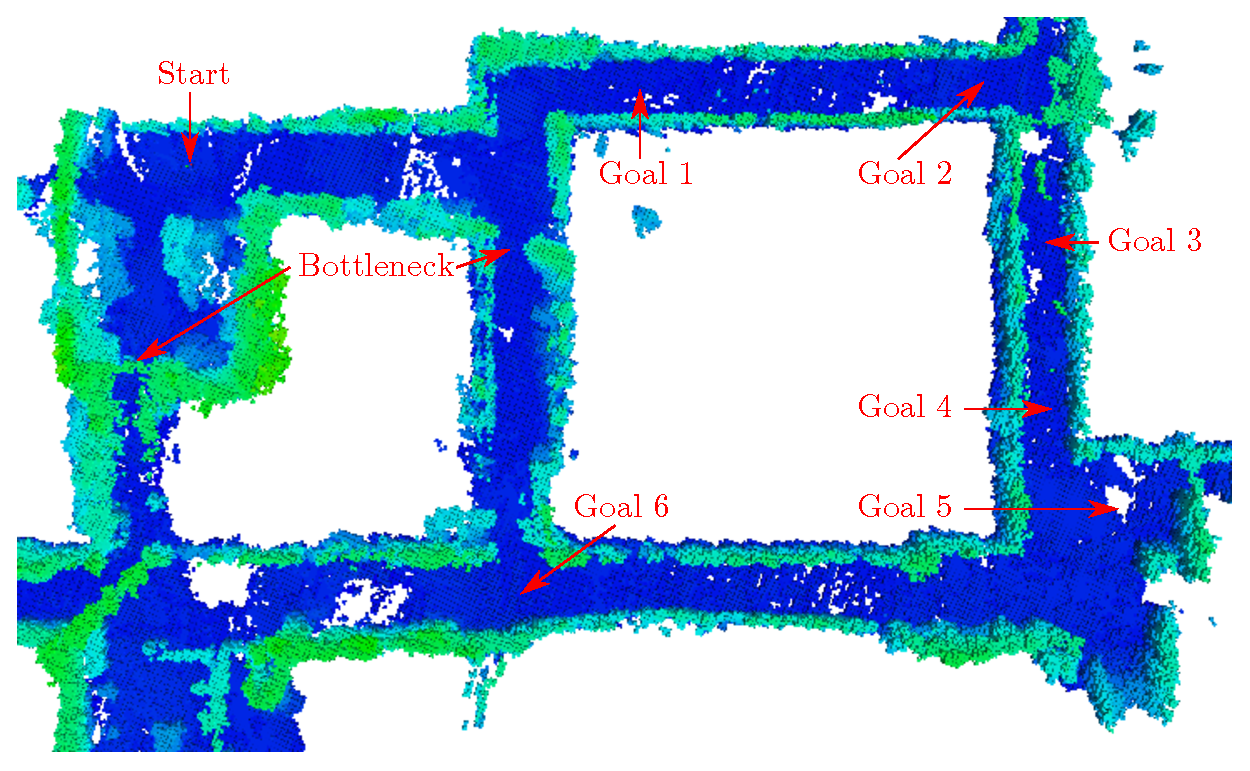
\includegraphics[trim = 0mm 86mm 94mm 0mm,clip,width=0.8\textwidth]{pics/ML4.eps}
   \caption{Bird's eye perspective on a hallway in the "ML" building of the ETH Zurich. The start and the end point are illustrated.}
   \label{pic:differentGoalRRT}
\end{figure}

The size of the bounding box was $0.5m$ in all dimensions. The straight line connection was discretized in $0.3m$ steps. The radius for the Ray Check was $0.5m$ and the points were place every 0.2 radian. The comparison has been performed for $\gamma = 1$ and $\gamma = 1.5$. All the combinations have been executed 10 times and the average computational times are listed in the following table:





\begin{table}[H] 
\begin{center}
    \begin{tabular}{ | c | c | c |}
    \hline
    Approach &  Time for $\gamma = 1$ &  Time for $\gamma = 1.5$ \\ \hline
    Bounding Box & $0.343s$  & $0.643s$  \\ \hline
    Ray Check & $0.473s$ & $1.233s$ \\
    \hline
    \end{tabular}
\caption{Average computational time for the two approaches "Bounding Box" and "Ray Check".}
    \label{tab:RayCheck}
\end{center}
\end{table}

As can bee seen, the Bounding Box approach performs better, independent of the $\gamma$ parameter. Anyway, the difference gets more significant if $\gamma$ and therefore the amount of rewiring increases.\newline

The Bounding Box approach performs better according to table \ref{tab:RayCheck} and does not have any problems with floating objects. Therefore, only the Bounding Box approach is applied further on. 





%\begin{figure}[h]
%   \centering
%   \includegraphics[width=1\textwidth]{pics/MapLine.png}
%   \caption{Ein Bild.}
%\end{figure}



%\begin{figure}[h]
%   \centering
%   \includegraphics[width=1\textwidth]{pics/initialSolution.png}
%   \caption{Ein Bild.}
%\end{figure}
%
%
%\begin{figure}[h]
%   \centering
%   \includegraphics[width=1\textwidth]{pics/Vertex_in_middle_2.png}
%   \caption{Ein Bild.}
%\end{figure}
%
%\begin{figure}[h]
%   \centering
%   \includegraphics[width=1\textwidth]{pics/section.png}
%   \caption{Ein Bild.}
%\end{figure}
%
%
%\begin{figure}[h]
%   \centering
%   \includegraphics[width=1\textwidth]{pics/Nlopt_after_sectionAndTime.png}
%   \caption{Ein Bild.}
%\end{figure}